%\documentclass[../IntroSensors.tex]{subfiles}
%\graphicspath{{\subfix{../images/}}}
%\begin{document}
  \setchapterstyle{kao}
  \setchapterpreamble[u]{\margintoc}
  \chapter{Build Instructions for MS5803 Pressure Sensor}
  \labch{ms5803}

  \begin{kaobox}[backgroundcolor=\SNcolor,frametitlebackgroundcolor=\SNcolor,frametitle=Estimated build time] Approximately two hours, plus 3D printing and epoxy set time.
  \end{kaobox}

  This chapter provides detailed instructions for building and waterproofing a \texttt{MS5803} pressure sensor. Code is provided for interfacing with the \texttt{MS5803-05BA} sensor, but it can be adapted for other sensors in the \texttt{MS5803} line. For measurements intended for water depths no greater than approximately 10 meters, a \texttt{MS5803-02} sensor is somewhat more precise.

  %\todo{Images still need to be uploaded to PublicSensors. WL 10/9/21}

  \begin{marginfigure}[1cm]
  	\begin{center}
      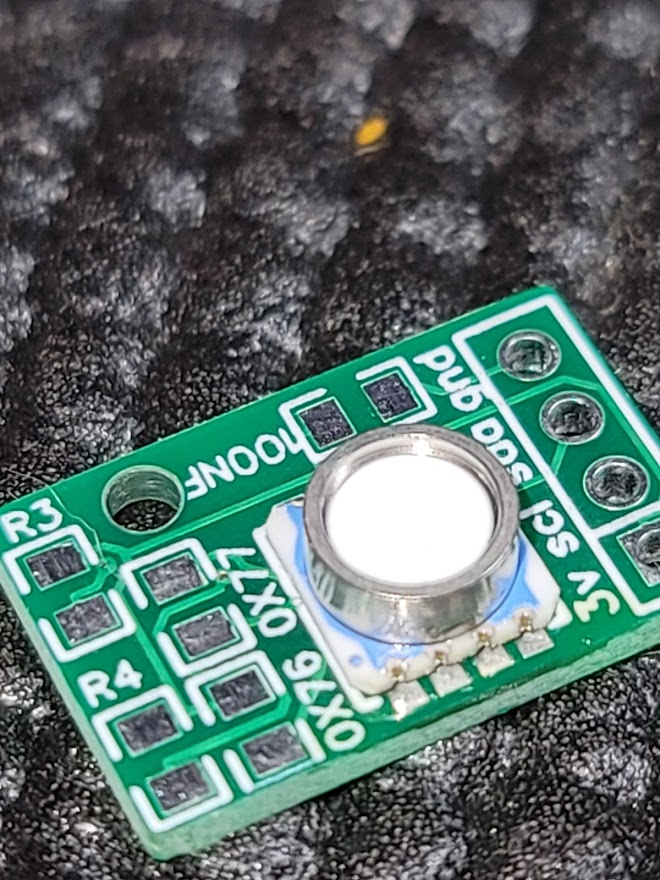
\includegraphics[width=\MFW]{Images/AppendixB_PCB2.jpg}
  		\caption[\texttt{MS5803-05} on PCB]{The sensor must be installed on a custom PCB before use.}
  		\labfig{PCB_2}
  	\end{center}
  \end{marginfigure}

  \begin{marginfigure}[9cm]
  	\begin{center}
      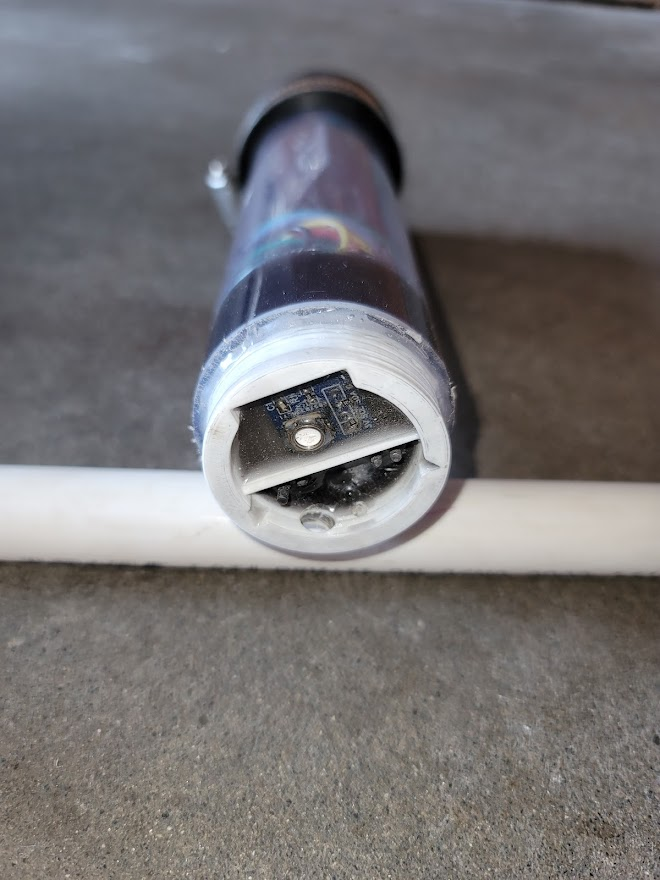
\includegraphics[width=\MFW]{Images/AppendixB_finished.jpg}
  		\caption[Finished Sensor]{The \texttt{MS5803} sensor is shown at the top.  The optional electrical conductivity electrodes are shown at bottom. Build instructions for the electrical conductivity device are provided elsewhere in this textbook.}
  		\labfig{finished}
  	\end{center}
  \end{marginfigure}

  \section{Materials and Equipment}
  The \texttt{MS5803} sensor is available only as a surface mount device, so it must be mounted to a circuit board before use, as shown in \reffig{PCB_2}. A procedure for accomplishing this without using a custom board is described at \htmladdnormallink{the Cave Pearl Project}{https://thecavepearlproject.org/2014/03/27/adding-a-ms5803-02-high-resolution-pressure-sensor/}. The build can be simplified if the device is installed on a PCB that includes the requisite pull-up resistors and decoupling capacitor. The design for such a board is available on \htmladdnormallink{GitHub}{https://github.com/jwlauer/CTD/tree/master/hardware/MS5803}. Multiple boards can be ordered for a minimal cost from manufacturers such as OSHPark or JLCPCB.
  These instructions assume that a waterproof housing is required. The housing is most easily built using a 3D printed cap into which the sensor will be installed and potted. The cap used in this build can also be used to house electrical conductivity electrodes as described elsewhere in this text. A finished version with both pressure sensor and conductivity electrodes is shown in as shown in \reffig{finished}. If a waterproof housing is not required, the build can be accomplished with only the PCB and \texttt{MS5803} sensor.

  \begin{kaobox}[frametitle=Soldering Surface Mount Devices]
  	Surface mount device (SMD) components are soldered directly to exposed metal pads on printed circuit boards. While the small size of the pads may seem intimidating at first, placing and soldering SMD parts is actually quite straightforward. Perhaps the best way to learn SMD soldering is to watch one of the many videos on the subject. Great tutorials have been developed by \htmladdnormallink{AdaFruit}{https://youtu.be/QzoPxvIM2qE}, \htmladdnormallink{SparkFun}{https://www.sparkfun.com/tutorials/96}, and a number of YouTube channels such as those by \htmladdnormallink{Mr SolderFix}{https://youtu.be/EW9Y8rDm4kE} or \htmladdnormallink{NematicsLab}{https://youtu.be/EW9Y8rDm4kE}. In this build, the biggest challenge is mounting the MS5803 sensor. Thankfully, metalic pads run up the sides of the MS5803 chips, making it relatively easy to see when a solder connection has formed. It is helpful to practice on a few SMD resistors first, and it is wise to have solder wick and flux on hand to repair any solder bridges, but soldering a \texttt{MS5803} is a doable project for anyone with a little through-hole soldering experience.
  \end{kaobox}

  \subsection{Materials}
  For a fully waterproof build, the following are required.

  \begin{table}[H]
  	\centering
  	\caption{Materials and supplies.} \label{tab:materials}
  	\begin{tabular}{|N|r|l|}
  		\hline
  		\multicolumn{1}{|c}{Number} & Item & Link  \\ \hline
  		\label{mat:MS5803} & \texttt{MS5803-05BA} sensor & \htmladdnormallink{URL}{https://www.te.com/usa-en/product-CAT-BLPS0011.html} \\
  		\label{mat:MS5803} & OR \texttt{MS5803-05BA} breakout & \htmladdnormallink{URL}{https://www.te.com/usa-en/product-CAT-BLPS0011.html} \\
      \label{mat:PCB} & Microcontroller, battery, \& waterproof enclosure & \\
  		\label{mat:PCB} & Custom PCB for \texttt{MS5803} & \htmladdnormallink{URL}{https://github.com/jwlauer/CTD/tree/master/hardware/MS5803} \\
  		\label{mat:usb_cbl} & 3D-printed cap & \htmladdnormallink{URL}{https://github.com/jwlauer/CTD/tree/master/hardware/3d_print}\\
  		\label{mat:pipe} & PVC Pipe (2-inch diameter) &  \\
  		\label{mat:wire} & Hookup wire (red, black, yellow, green) &  \\
  		\label{mat:rsts} & 10,000 Ohm SMT Resistors (0805 or 1206 footprint) &  \\
  		\label{mat:leds} & 100 nF capacitor (0805 or 1206 footprint) & \\
      \label{mat:pot} & Electronic Potting Compound (e.g., EpoxySeal 9000) & \\
      \label{mat:polish} & Clear Nail Polish (for initial seal of 3D print) & \\
      \label{mat:glue} & 5-minute epoxy (for gluing 3D-printed cap to PVC) & \\
      \label{mat:pins} & Male Header Pins & \\
      \label{mat:dupont} & Crimpable 2.54 Pitch Dupont Connectors & \\
      \label{mat:dupont} & Solder flux pen & \\
      \label{mat:dupont} & Solder wick & \\
      \hline
  	\end{tabular}
  \end{table}

  \subsection{Equipment}

  \begin{table}[H]
  	\centering
  	\caption{Equipment.} \label{tab:materials}
  	\begin{tabular}{|N|r|l|}
  		\hline
  		\multicolumn{1}{|c}{Number} & Item & Link  \\ \hline
  			\label{eq:crimper} & wire crimpers & \htmladdnormallink{URL}{https://iwiss.com/?gclid=Cj0KCQjw-4SLBhCVARIsACrhWLVIyvwrUxixiFN2eDen8ME2A0kMXZ9P9J6lTcpAKf9vG4RkeLrV4nUaAsLBEALw_wcB} \\
        \label{eq:solder} & Soldering iron w/ fine tips & \\
        \label{eq:tray} & Flat surface to contain spilled epoxy & \\
        \label{eq:pvccutter} & Hacksaw or PVC cutting tool & \\
        \label{eq:hand} & Helping hands \& magnifying glass & \\
        \label{eq:tweezers} & Steel tweezers for placing SMD parts & \\
        \hline
  	\end{tabular}
  \end{table}

  \section{Build Instructions}

  \begin{marginfigure}
  	\begin{center}
      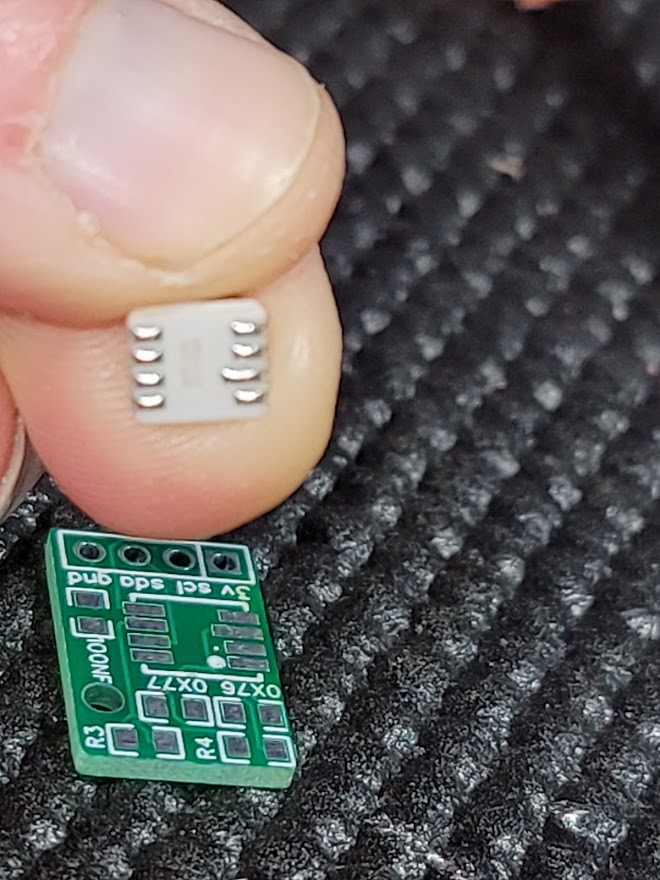
\includegraphics[width=\MFW]{Images/AppendixB_PCB.jpg}
  		\caption[Alignment for \texttt{MS5803}]{Align the longer pad on the sensor with the longer pad on the PCB.}
  		\labfig{PCB_1}
  	\end{center}
  \end{marginfigure}

  \begin{enumerate}
  	\item Order PCB from a PCB supplier based on files at \htmladdnormallink{GitHub}{https://github.com/jwlauer/CTD/tree/master/hardware/MS5803} or \htmladdnormallink{OSHWLab}{https://oshwlab.com/WesLauer/ms5803_pullups_copy}. Provide several weeks for shipping.
    \item Print 3D cap from STL file on \htmladdnormallink{GitHub}{https://github.com/jwlauer/CTD/tree/master/hardware/MS5803}. There are two versions of the cap--one designed to fit inside 2-inch nominal PVC pipe and one designed to fit over 1-inch nominal PVC pipe. The 2-inch cap incudes room for the optional electrical conductivity electrodes; the 1-inch size does not. Photographs here illustrate the 2-inch version.
    \item Solder sensor to PCB in position shown in \reffig{PCB_1}, with the longer pad on the sensor aligned with the longer pad on the PCB. There are many videos on YouTube that provide guidance on soldering SMT parts. Stabilizing the PCB with masking tape or helping hands and using tweezers to stabilize the part while soldering is usually enough to allow the devices to be soldered by hand. It is often helpful to liberally apply flux to both the part and pads on the circuitboard with a flux pen before soldering.
    \item Solder 10KOhm SMT resistors to pads R3, R4, and either pads 0x76 or 0x77, which define the I2C address of the device. This textbook assumes the device is at address 0x76.
    \item Solder 100 nF SMT capacitor to the 100NF pad.
  	\item Solder male headers to PCB so that headers are oriented downward.
    \item Test the device by wiring to the microcontroller according to the instructions at the end of this chapter.  Make sure the device produces believable data before proceeding with the build.
  	\item Place male headers through openings in 3D-printed cap (\reffig{cap}) and solder 40 cm of wire to each headers. The color scheme used in this text is red-->3V, black-->ground, yellow-->scl, green-->sda.
  	\item Crimp DuPont connectors to each of the four wires.

    \begin{marginfigure}
      \begin{center}
        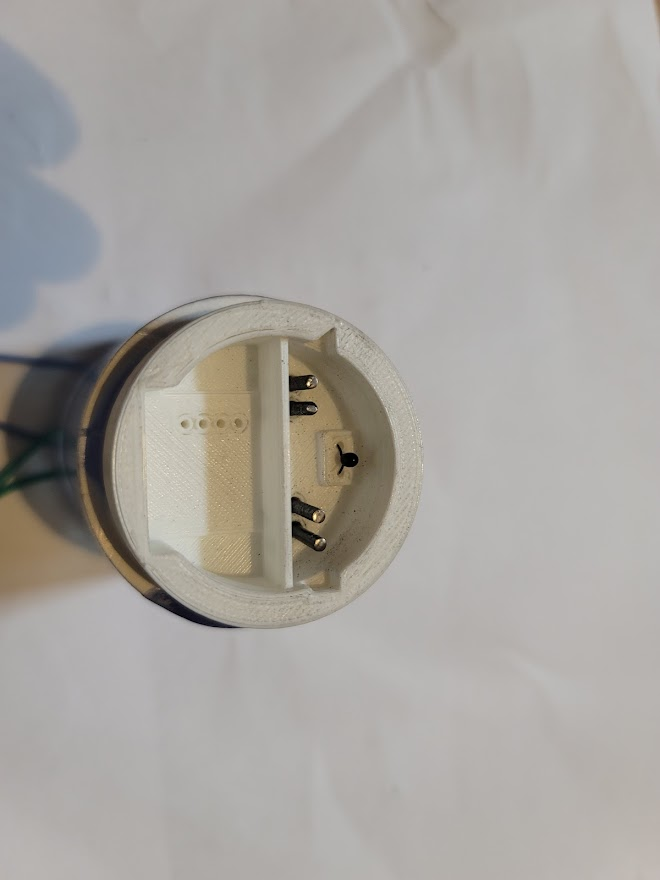
\includegraphics[width=\MFW]{Images/AppendixB_cap.jpg}
        \caption[3D-Printed Cap]{Electrical connections for the MS5803 are made by placing header pins through the four small holes at left. Optional electrical conductivity electrodes and thermistor are visible at right.}
        \labfig{cap}
      \end{center}
    \end{marginfigure}

    \item Optional: If building the electrical conductivity sensor described elsewhere in this textbok, install electrodes in 3D printed housing.
    \item Cut PVC pipe to desired length. If the microcontroller is intended to be placed inside the PVC pipe and enclosed with a flexible rubber cap, the pipe length should be long enough to include both the microcontroller batteries, so perhaps 30 cm.  If the microcontroller will be housed in a separate pipe, the PVC can be much shorter--perhaps 5 or 10 cm.
    \item Use a quick setting epoxy to glue the cap into the PVC pipe (\reffig{mount}) and to seal any remaining space where the header pins pass through the cap. It is helpful if the entire bottom of the 3D printed cap is painted with the epoxy to ensure that the cap can hold the potting epoxy used later. If EC electrodes are going to be used, be sure these are installed before sealing the bottom of the cap and gluing into place.

    \begin{marginfigure}
    	\begin{center}
        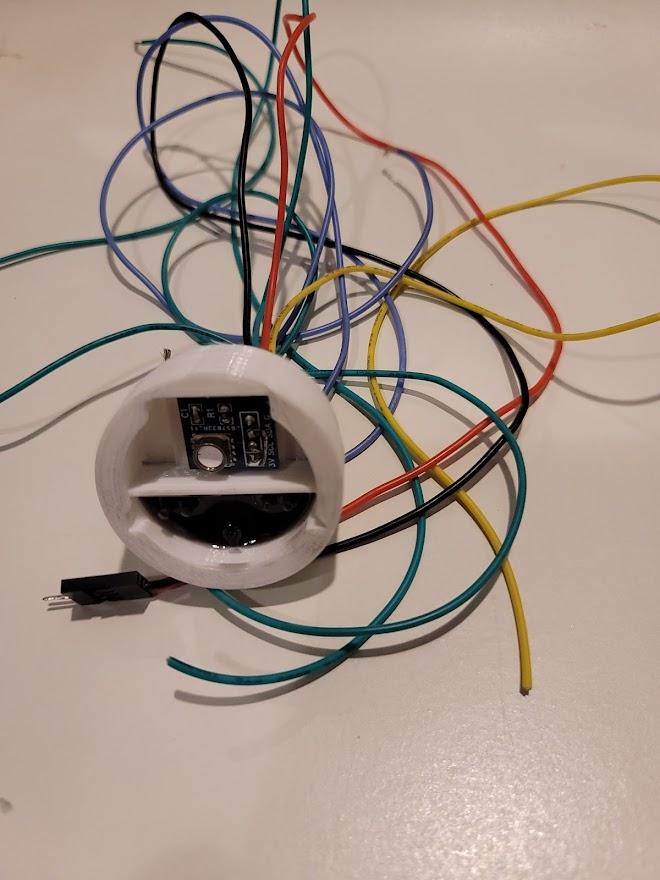
\includegraphics[width=\MFW]{Images/AppendixB_mount_in_cap.jpg}
    		\caption[Mounting for \texttt{MS5803}]{Once installed, the sensor should sit flush on the 3D printed housing. In this image, potting compount has been placed around the optional electrical conductivity electrodes, and wires from these electrodes, the thermistor, and the MS5803 are visible.}
    		\labfig{mount}
    	\end{center}
    \end{marginfigure}

    \item Use clear nail polish to seal the outside of the 3D printed cap.  Wait for this to dry before moving on.
  	\item For this step, the device should be placed over a surface such as newspaper that can handle spilled potting compound. Stabilize the device so that the top of the metal ring around the MS5803 sensor is perfectly level. Then mix potting compound according to manufacturer's directions and CAREFULLY pour into the space around the sensor such that the potting fluid fully encases all electronics but does NOT flow onto the sensor itself.
  	\item Let potting fluid set for the manufacturer-recommended period (e.g., overnight). Note that for some potting fluids, setting time can be reduced if temperature is kept artificially high, but this can affect the integrity of the PVC pipe or 3D printed housing if care is not taken to prevent overheating.
    \item After the potting compound around the sensor is fully set, turn the device over and fill the inside of the pipe with several cm of potting compound. Be careful not to get any compound on the top or outside of the pipe because this could affect the waterproofness of the seal that will be made with the cap. Once the potting compound inside the device has cured, the sensor is ready for use.
  \end{enumerate}

  \subsection{Wiring to microcontroller}
  The \texttt{MS5803} is an I2C device, so it simply needs to be wired to the I2C bus on the microcontroller. The code presented here assumes SCL is attached to Pin 22, SDA to Pin 21, 3V is connected to a 3.3 volt output from the microcontroller, and GND is connected to ground. However, the MS5803 driver allows any GPIO pin to serve the role of power and ground pins. Using GPIO pins in this way can simpify a build because it allows all four wires to be connected to contiguous GPIO pins on the microcontroller. It also allows the device to be completely de-powered during sleep simply by putting the power pin into a digital low state.

  \subsection{Code and testing}
  Copy ms5803.py to the microcontroller. Then execute the following code.

  \subsection{\lstinline{ms5803_test.py}}
  \lstinputlisting[language=Python,label=ms5803_test,caption={Test code for the \texttt{MS5803\_05} pressure and temperature sensor.}]{Codes/ms5803_test.py}

  \subsection{\lstinline{ms5803.py}}
  \lstinputlisting[language=Python,label=ms5803,caption={Driver for the \texttt{MS5803\_05} pressure and temperature sensor.}]{Codes/ms5803.py}

  Modified from \htmladdnormallink{ms5803\_05BA.py}{https://github.com/ControlEverythingCommunity/MS5803-05BA/blob/master/Python/MS5803_05BA.py}, distributed at \htmladdnormallink{Control Everything github repository}{https://github.com/ControlEverythingCommunity}.
%\end{document}
